% !TEX root =  ../report.tex

\section{Testing}
Throughout development, an example application was used to test code generation, and verify the results. The application has been used previously for validating generated OP2 code, as it makes use of all the key features, including having both direct and indirect loops. It is called \textit{airfoil}, and is a computational fluid dynamics solver which models the air flow around the cross section of a aeroplane wing, using unstructured grid to discretise the space. A document detailing the airfoil code is available on the OP2 website \cite{airfoil}.

\subsection{Test Plan}
Since the project is centered around code generation, the generated code must of course be valid - and compile without error. It is possible this could vary between compilers, so in this report results are primarily gathered using the Intel C/C++ Compilers, and the Intel MPI library. The Nvidia C Compiler \verb|nvcc| is used to compile the CUDA device code sections, but it will refer all host code compilation to \verb|icpc|.
\par
Once the generated code compiles successfully, the most important result to achieve is that the compiler executable creates an output that is within tolerance of the expected value. Performance is still important - and the goal of this project is to investigate whether this technique does provide any performance benefit - but any perfomance increase that incurs unaccebtable deviation from the expected result is not a useful benefit. Section TODO on Benchmarking will cover the performance analysis.
\par
With this in mind, the airfoil application code includes a test of the result after 1000 iterations against the expected outcome, and prints the percentage difference. A difference of less than 0.00001 is considered within tolerance due to the potential for minor floating point errors, and therefore a passing test.
\par
The initial state for the test is a folder with the files listed in Figure \ref{fig:files_a} (p\pageref{fig:files_a}). The main application file is \verb|airfoil.cpp| which contains OP2 API calls, and the structure of the program. The 5 header files contain the user functions for the respective parallel loop with the same name, and \verb|new_grid.h5| is the input data in the Heterogenous Data Format (HDF5 \cite{HDF5}) file format.

\subsection{Test Results}

\subsubsection{Code Generation}
To test the code generation, the python script \verb|op2.py| is called in the directory, passing the main application file \verb|airfoil.cpp| as an argument, as well as the string \verb|JIT| to make sure the correct code generation scripts are called.
\codeline{ python2 \$OP2_INSTALL_PATH/../translator/c/python/op2.py airfoil.cpp JIT}{}
\noindent After running this command, the expected outcome is that a new file: \verb|airfoil_op.cpp| is created in the directory, and a directory named \verb|cuda/| will be created with eleven files in it: Two for each of the five parallel loops, as described in Section \ref{sec:codegen}; and a single master kernels file named \verb|airfoil_kernels.cu|.
\par
This test is considered a pass if these files exist, as their contents is validated as correct by the next tests passing. A folder called \verb|seq/| is also created by the translator script\\
 \verb|translator/c/python/jit/op2_gen_seq_jit.py|, which was not completed as part of this project, but part of the \verb|feature/lazy-execution|, the parent branch of \verb|feature/jit|.
 \\\\
 \setlength{\fboxsep}{1em}
 \fbox{%
  \parbox{\textwidth}{%
    Figure \ref{fig:files_b} shows the folder after running the above command. The test is considered \textbf{\textcolor{green!20!black}{PASSED}}.
  }%
}

\subsubsection{Ahead-of-Time Compilation}


\subsubsection{Just-in-Time Compilation}

\subsubsection{Output}

\begin{figure}[t!p]
\centering     %%% not \center
\caption{Files in Application Folder}
\subfloat[Input Files]{\label{fig:files_a}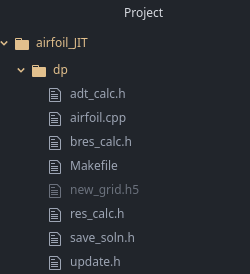
\includegraphics[width=60mm]{files1}}
 \qquad
\subfloat[After Code Generation]{\label{fig:files_b}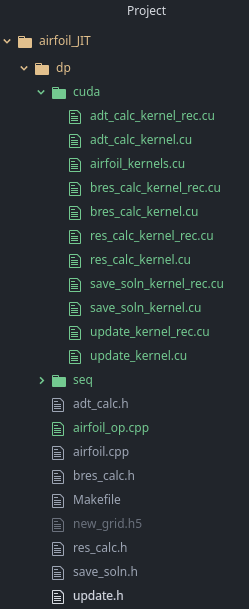
\includegraphics[width=60mm]{files2}}
\vspace*{3in}
\end{figure}

\begin{figure}[tp]\ContinuedFloat
\centering     %%% not \center
\caption{Files in Application Folder}
\subfloat[After AOT Compile]{\label{fig:files_c}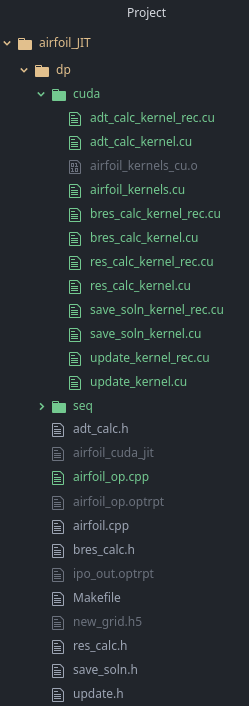
\includegraphics[width=60mm]{files3}}
 \qquad
\subfloat[After Execution]{\label{fig:files_d}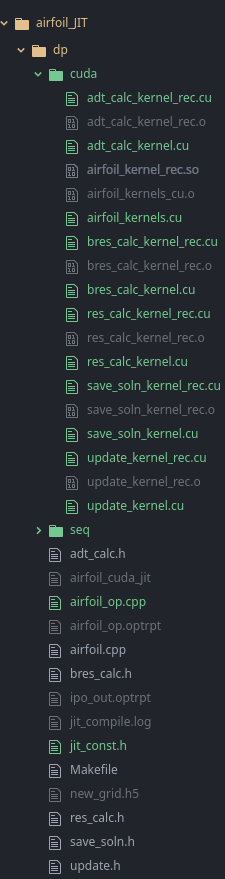
\includegraphics[width=60mm]{files4}}
\end{figure}
